\chapter{Systemmodelle}



\section{Szenarien}

\subsubsection*{Akteure}

\begin{tabular}{lp{0.9\linewidth}}

Alice & Der Benutzer des Programms \programname. \\

Bob & Der Angreifer des Firmennetzwerkes. \\

Insekura & Die Firma dessen Geräte ProfiNet zur internen Kommunikation verwenden. \\

\programname & Die Software zur Beobachtung der Netzwerkkommunikation.\\

\end{tabular}

\subsection{Szenario 1: Hinzufügen von erlaubten Adressen}

Alice's Firma Insekura nutzt das industrielle Protokoll ProfiNet für die Kommunikation zwischen den Geräten des Systems. Bisher hat Alice keine Möglichkeit gehabt den Netzwerkverkehr zwischen den Drehmaschinen zu kontrollieren. Während des laufenden Betriebs greift der ehemalige Mitarbeiter Bob unbeobachtet auf den Maschinenablauf zu und verursacht dadurch eine Werkzeugkollision. Der materielle Schaden für die Firma ist groß, ein Mitarbeiter wurde leicht verletzt. Zudem kann Alice den Ablauf der Kommunikation und damit die Ursache des Schadens nicht zurückverfolgen.

In der Hoffnung Unfälle und Attacken solcher Art in Zukunft vermeiden zu können, installiert sie die freie Software \programname und lässt sie auf einem gut sichtbaren Bildschirm in ihrem Büro dauerhaft in Betrieb. Auf dem Display sieht sie sämtliche \textbf{Geräte als Knoten} eines Graphen und kann die \textbf{Kommunikationswege zwischen Geräten und Controllern durch gerichtete Kanten} gut verfolgen. In den Einstellungen von \programname \textbf{fügt sie den Adressraum des Firmennetzes zu den erlaubten Kommunikationsadressen hinzu}.

\subsection{Szenario 2: Echtzeit Beobachtung von Angriffen}

Im Laufe der nächsten Tage startet Bob einen weiteren Versuch seiner alten Firma zu schaden. Letztes Mal hat das wunderbar funktioniert, keiner konnte seine fremde Adresse identifizieren und er hatte uneingeschränkte Möglichkeiten falsche Daten an die Drehmaschinen zu übermitteln.

Während sich Bob den Zugang auf das System verschafft, sitzt Alice in ihrem Büro und hat ihren Blick gerade auf den Bildschirm mit dem laufenden \programname gerichtet. Sie sieht wie ein roter Knoten auf dem Bildschirm erscheint und mit einer der Drehmaschinen beginnt zu kommunizieren. Die Kommunikationskante ist auch rot gekennzeichnet. Sofort eilt Alice zur Tür und drückt auf den Notfall Ausschalter des Systems. Schlimmeres konnte verhindert werden.

\subsection{Szenario 3: Auslesen von Log Dateien}

Alice öffnet die log Datei des roten Knotens, der den Angriff gestartet hat und kann dadurch zurückverfolgen wer sich unerlaubten Zugriff auf das Firmennetzwerk verschafft hat. Bob steht eine große Schadensersatzklage bevor.


\section{Anwendungsfälle}

\subsection{Markieren von Adressen und Namen}

\begin{tabular}{lp{0.9\linewidth}}

\textbf{Name} & Anpassen erlaubter/unerlaubter Adressen und Namen \\

\textbf{Teilnehmender Akteur} & Benutzer \\

\textbf{Eingangsbedingung} &
				\begin{minipage}[t]{\linewidth}
				\begin{itemize}[nosep,after=\strut,leftmargin=10pt]

				\item \programname und Snort mit \sppname sind in Betrieb

				\end{itemize}
				\end{minipage} \\
\textbf{Ereignisfluss} &
				\begin{minipage}[t]{\linewidth}
				\begin{itemize}[nosep,after=\strut,leftmargin=10pt]

				\item Benutzer navigiert ins Einstellungsmenü
				\item Benutzer passt die gewünschte Liste an
				\item Benutzer bestätigt Änderungen

				\end{itemize}
				\end{minipage} \\

\end{tabular}

\subsection{Netzwerkaktivität beoboachten}

\begin{tabular}{lp{0.9\linewidth}}
\textbf{Name} & Netzwerkaktivität beobachten \\

\textbf{Teilnehmender Akteur} & Benutzer \\

\textbf{Eingangsbedingung} &
				\begin{minipage}[t]{\linewidth}
				\begin{itemize}[nosep,after=\strut,leftmargin=10pt]

				\item \programname und Snort mit \sppname sind in Betrieb
				\item Aktiver Datenverkehr zwischen Geräten des Netzwerkes

				\end{itemize}
				\end{minipage} \\
\textbf{Ereignisfluss} &
				\begin{minipage}[t]{\linewidth}
				\begin{itemize}[nosep,after=\strut,leftmargin=10pt]

				\item Benutzer beobachtet und interagiert mit der Benutzeroberfläche
				\end{itemize}
				\end{minipage} \\

\end{tabular}

\subsection{Graph skalieren}

\begin{tabular}{lp{0.9\linewidth}}
\textbf{Name} & Graph skalieren \\

\textbf{Teilnehmender Akteur} & Benutzer \\

\textbf{Eingangsbedingung} &
				\begin{minipage}[t]{\linewidth}
				\begin{itemize}[nosep,after=\strut,leftmargin=10pt]

				\item \programname und Snort mit \sppname sind in Betrieb
				\item Aktiver Datenverkehr zwischen Geräten des Netzwerkes

				\end{itemize}
				\end{minipage} \\
\textbf{Ereignisfluss} &
				\begin{minipage}[t]{\linewidth}
				\begin{itemize}[nosep,after=\strut,leftmargin=10pt]
				\item Benutzer dreht das Mausrad
				\end{itemize}
				\end{minipage} \\
\end{tabular}

\subsection{Einstellungen speichern}

\begin{tabular}{lp{0.9\linewidth}}
\textbf{Name} & Graph skalieren \\

\textbf{Teilnehmender Akteur} & Benutzer \\

\textbf{Eingangsbedingung} &
				\begin{minipage}[t]{\linewidth}
				\begin{itemize}[nosep,after=\strut,leftmargin=10pt]

				\item \programname und Snort mit \sppname sind in Betrieb

				\end{itemize}
				\end{minipage} \\
\textbf{Ereignisfluss} &
				\begin{minipage}[t]{\linewidth}
				\begin{itemize}[nosep,after=\strut,leftmargin=10pt]
				\item Benutzer navigiert ins Einstellungsmenü
				\item Benutzer klickt auf den "Einstellungen speichern" Eintrag
				\end{itemize}
				\end{minipage} \\
\end{tabular}

\subsection{Programm beenden}

\begin{tabular}{lp{0.9\linewidth}}
\textbf{Name} & Graph skalieren \\

\textbf{Teilnehmender Akteur} & Benutzer \\

\textbf{Eingangsbedingung} &
				\begin{minipage}[t]{\linewidth}
				\begin{itemize}[nosep,after=\strut,leftmargin=10pt]

				\item \programname und Snort mit \sppname sind in Betrieb

				\end{itemize}
				\end{minipage} \\
\textbf{Ereignisfluss} &
				\begin{minipage}[t]{\linewidth}
				\begin{itemize}[nosep,after=\strut,leftmargin=10pt]
				\item Benutzer navigiert ins File Menü
				\item Benutzer klickt auf den Eintrag "Exit"
				\item Benutzer wird gefragt ob Einstellungen gespeichert werden sollen
				\item Programm wird beendet
				\end{itemize}
				\end{minipage} \\
\end{tabular}

\pagebreak

\subsection*{Anwendungsfalldiagramm - Benutzerinteraktion}

\begin{figure}[h!]
    \centering
    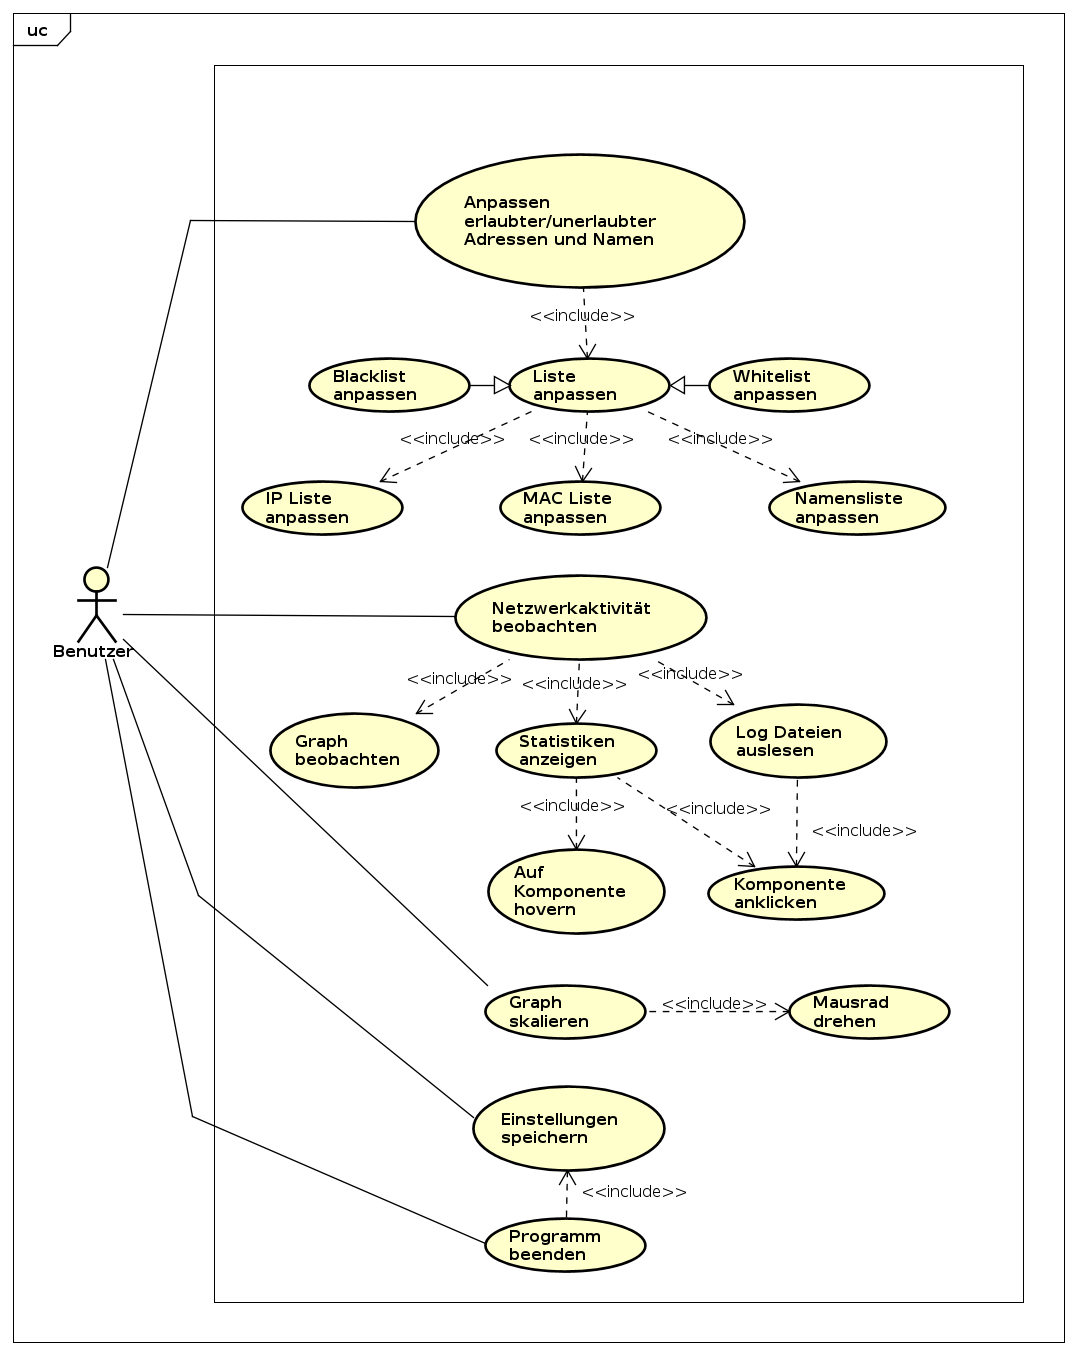
\includegraphics[width=\textwidth]{../diagrams/UC_Benutzerinteraktion.png}
    \caption{Anwendungsfalldiagramm Benutzerinteraktion}
\end{figure}

\pagebreak
\section{Dynamische Modelle}

	\subsection{Beschreibung: Programmablauf}

	\begin{easylist}[enumerate]
	\ListProperties(Style2*=,Numbers=a,Numbers1=R,FinalMark1={.},FinalMark2={.},FinalMark3={.},Numbers4=l)


	& \programname wird gestartet (siehe Grafik "Starte Programm")

	& \programname und \sppname laufen als getrennte Prozesse

		&& Prozess: Wenn Snort noch nicht läuft wird Snort gestartet und sendet Paketdaten an den \programname Prozess (siehe Grafik "Präprozessoraktivitäten")

		&& Prozess: \programname startet mehrere Threads

			&&& Kontrollfluss:
			&&&& Prüfen auf neue Pakete
			&&&& Vorhandenes Paket wird gelesen und aus dem Puffer gelöscht
			&&&& Paket wird verarbeitet wenn vorhanden (siehe Grafik "Verarbeite Paketdaten")

			&&& Kontrollfluss:
			&&&& \programname reagiert und verarbeitet Benutzerinteraktion (siehe Anwendungsfälle "Benutzerinteraktion")

			&&& Kontrollfluss:
			&&&& \programname empfängt Paketdaten von Snort und schreibt sie in den Prozessinternen Paketpuffer

	& Unabhängig voneinander wird die GUI nach jeder Veränderung durch neue Paketdaten oder Benutzereingaben aktualisiert
	& Das Programm wird bei Bedarf beendet

	\end{easylist}

	\pagebreak

  \begin{figure}[h!]
      \hspace*{0.15cm}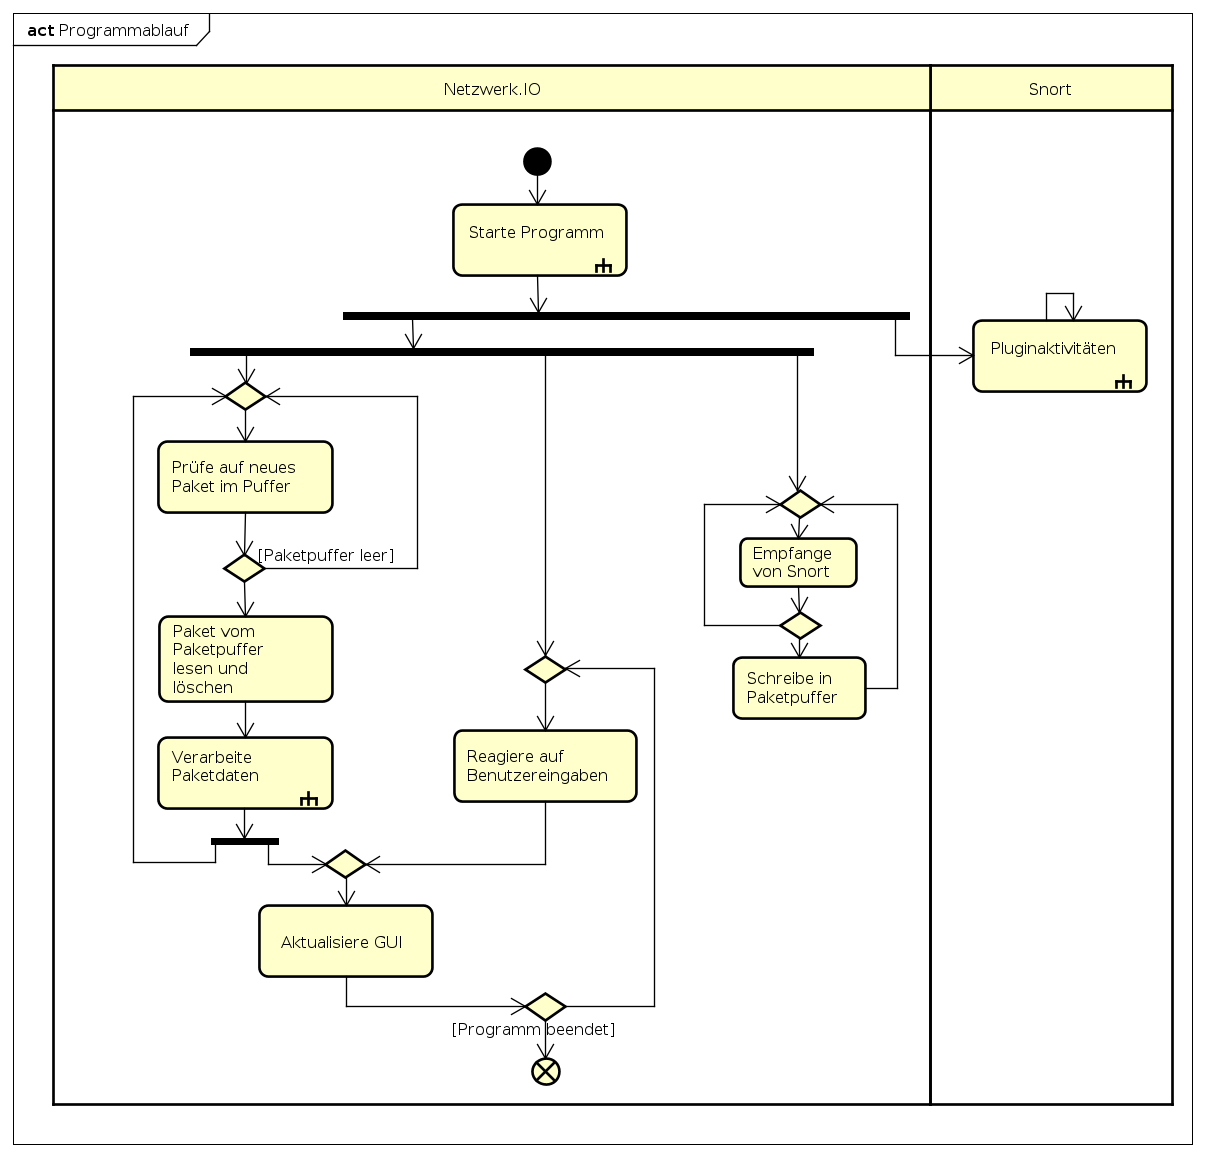
\includegraphics[width=\textwidth]{../diagrams/AD_Programmablauf}
      \caption{Aktivitätsdiagramm Programmablauf}
  \end{figure}

	\pagebreak
\subsection{Beschreibung: Starte Programm}

	\begin{easylist}[enumerate]
	\ListProperties(Style2*=,Numbers=a,Numbers1=R,FinalMark1={.},FinalMark2={.},FinalMark3={.},Numbers4=l)


	& Initialisiere relevante Daten

	& Wenn Snort noch nicht läuft, frage den Benutzer ob Snort gestartet werden soll
		&& Wenn der Benutzer zustimmt wird Snort mit dem Präprozessor gestartet
		&& Wenn der Benutzer ablehnt wird Netzwerk.IO beendet

	& Wenn Snort schon läuft, dann Benutzer fragen ob Präprozessor gestartet werden soll
	    && Wenn der Benutzer zustimmt wird Snort mit dem Präprozessor neu geladen
	    && Wenn der Benutzer nicht zustimmt wird Netzwerk.IO beendet

	\end{easylist}

    \begin{figure}[h!]
        \centering
        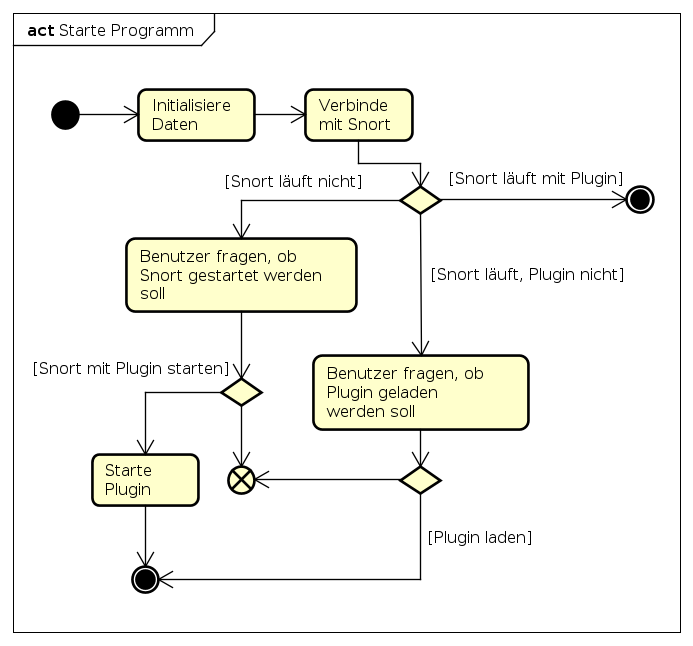
\includegraphics[width=\textwidth]{../diagrams/AD_Starte_Programm}
        \caption{Aktivitätsdiagramm Starte Programm}
    \end{figure}

\pagebreak
\subsection{Beschreibung: Präprozessoraktivitäten}

	\begin{easylist}[enumerate]
	\ListProperties(Style2*=,Numbers=a,FinalMark1={.},FinalMark2={.},FinalMark3={.},Numbers4=l)


	& Der Snort Präprozessor empfängt ein neues Paket
	& Das Paket wird dekodiert
	& Das dekodierte Paket wird auf Fehler geprüft
	    && Wenn ein Fehler gefunden wurde wird das Paket als fehlerhaft markiert
	& Das Paket wird an Netzwerk.IO weitergesendet
	& Das Paket wird für weitere Analysen auch an Snort weitergegeben

	\end{easylist}

    \begin{figure}[h!]
        \centering
        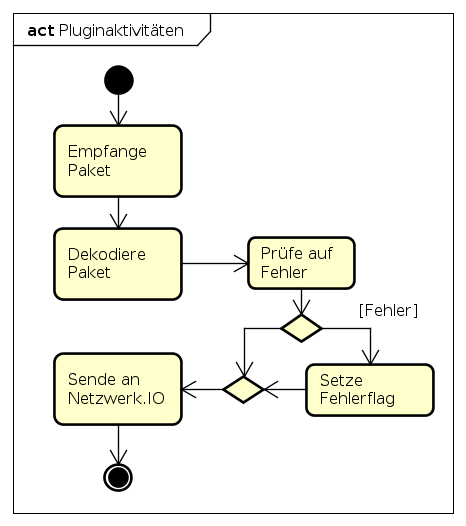
\includegraphics[width=0.5\textwidth]{../diagrams/AD_Praeprozessoraktivitaeten}
        \caption{Aktivitätsdiagramm Präprozessoraktivitäten}
    \end{figure}

\pagebreak
\subsection{Beschreibung: Verarbeite Paketdaten}

	\begin{easylist}[enumerate]
	\ListProperties(Style2*=,Numbers=a,Numbers1=R,FinalMark1={.},FinalMark2={.},FinalMark3={.},Numbers4=l)


	& Der Snort Präprozessor empfängt ein neues Paket
	& Das Paket wird dekodiert
	& Das dekodierte Paket wird auf Fehler geprüft
	    && Wenn ein Fehler gefunden wurde wird das Paket als fehlerhaft markiert
	& Das Paket wird an Netzwerk.IO weitergesendet
	& Das Paket wird für weitere Analysen auch an Snort weitergegeben

	\end{easylist}

    \begin{figure}[h!]
        \centering
        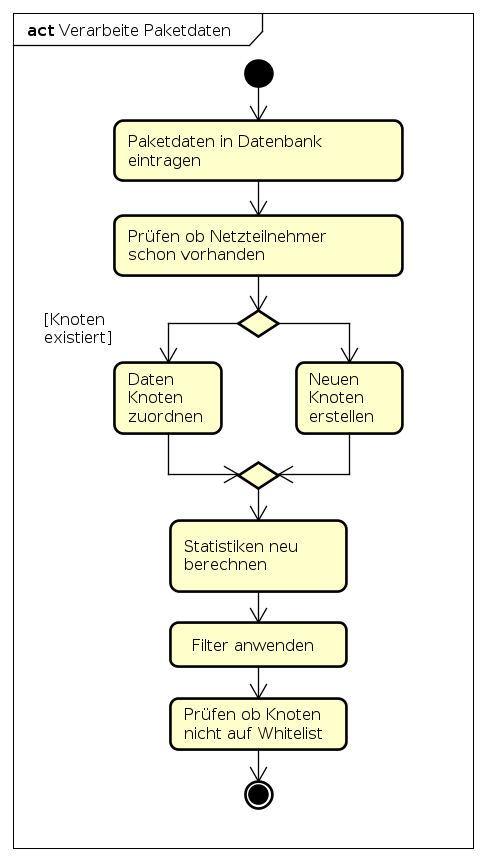
\includegraphics[width=0.5\textwidth]{../diagrams/AD_Verarbeite_Paketdaten}
        \caption{Aktivitätsdiagramm Verarbeite Paketdaten}
    \end{figure}

\section{Statische Modelle}

\subsection{Komponentenmodell}
\begin{easylist}[enumerate]
	\ListProperties(Style2*=,Numbers=a,Numbers1=R,FinalMark1={.},FinalMark2={.},FinalMark3={.},Numbers4=l)
    &Der Neztwerkverkehr erreicht Snort über einen Port und wird innerhalb von Snort von Komponente zu Komponente 
    &nach unten weiter bearbeitet. Unser einprogrammierter Präprozessor leitet die Pakete über die vordefinierte &Schnittstelle an den Controller von Netzwerk.IO, damit dieser entscheiden kann, wie die Pakete einzuordnen &sind. Des Weiteren gibt es eine optionale Schnittstelle eines Snort-Output-Plugins um die Alerts an den Controller des \programname weiter zu schicken.

	\end{easylist}
\begin{figure}[h!]
    \centering
    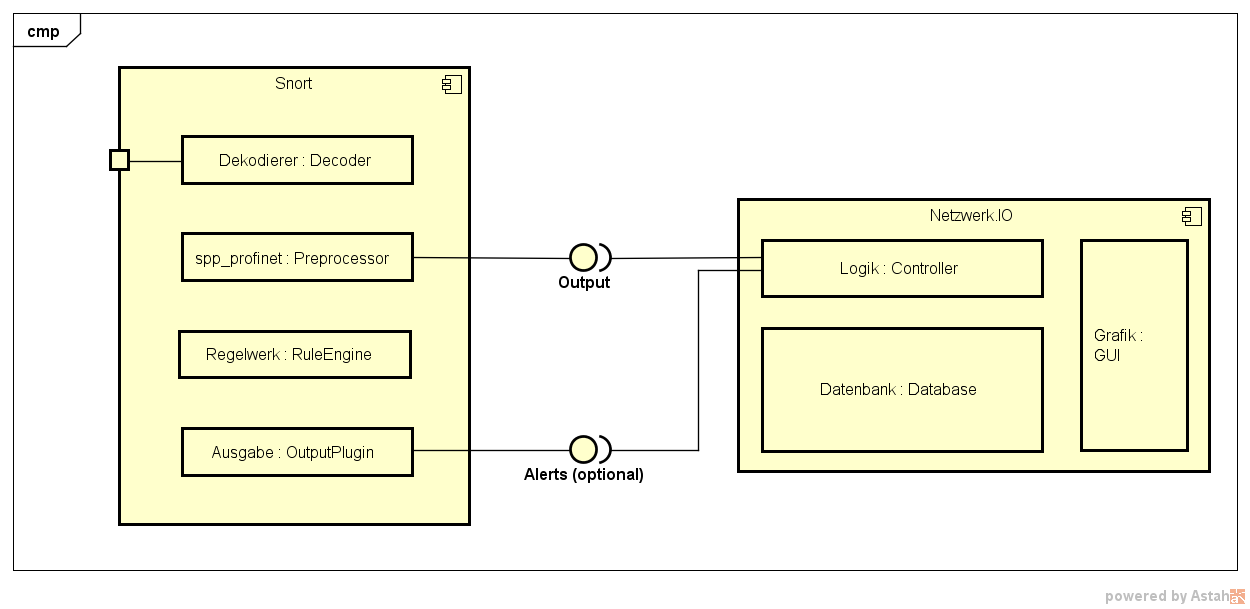
\includegraphics[width=\textwidth]{../diagrams/CMP_Architekturdiagramm.png}
    \caption{Komponentenmodell}
\end{figure}
